% !TEX root = ../main.tex
%---------------------------------------------------------------------------------------------------
%---------------------------------------------------------------------------------------------------
\section{Empirical setup}\addtocounter{framenumber}{-1}
%---------------------------------------------------------------------------------------------------
%---------------------------------------------------------------------------------------------------
\begin{frame}\frametitle{Eckstein--Keane--Wolpin models}

\begin{multicols}{2}

	\heading{Understanding individual decisions}\vspace{0.3cm}
	\begin{itemize}\setlength\itemsep{1em}
		\item Human capital investment
		\item Consumption--savings decision
	\end{itemize}

    \pause

	\heading{Predicting effects of policies}\vspace{0.3cm}
	\begin{itemize}\setlength\itemsep{1em}
		\item Educational policy
		\item Welfare programs
	\end{itemize}

\end{multicols}

\pause
\heading{Mathematical framework and implementation}\vspace{0.3cm}
\begin{itemize}\setlength\itemsep{1em}
 \item Finite-horizon discrete Markov decision problem
 \item Backward induction algorithm
\end{itemize}

\end{frame}
%---------------------------------------------------------------------------------------------------
%---------------------------------------------------------------------------------------------------
\begin{frame}{Timing of events}
\vspace{0.5cm}
\scalebox{0.9}{\hspace{-0.2cm}%!TEX root = ../main.tex
% \definecolor{gray}{RGB}{31,119,180}

% \definecolor{light-gray}{gray}{0.85}


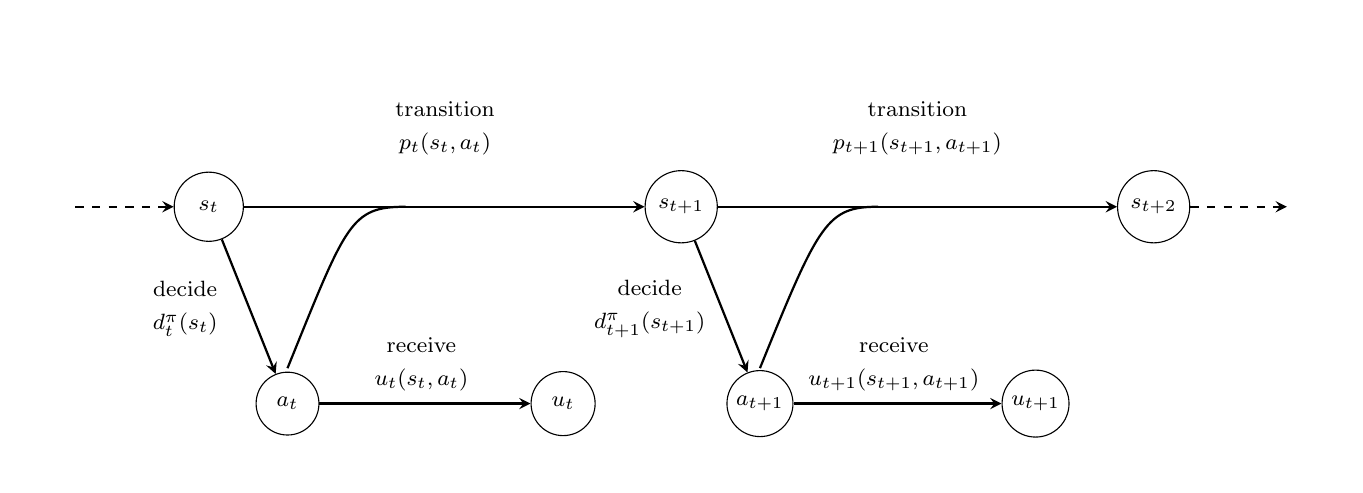
\begin{tikzpicture}[node distance=2cm]
%define styles
\tikzstyle{startstop} = [circle, rounded corners, minimum width=0.6cm, minimum height=0.3cm,text centered, draw=black]
[
->,
>=stealth',
auto,node distance=3cm,
thick,
main node/.style={circle, draw, font=\sffamily\Large\bfseries}
]
\tikzstyle{arrow} = [thick,->,>=stealth]]
\tikzstyle{darrow} = [dotted,->,>=stealth]]
%first and second column

\node (r0) [startstop, xshift = -3cm, draw = none] {};
\node (r999) [startstop, xshift = 13cm, draw = none] {};

\node (r1) [startstop, xshift = -1cm] {\footnotesize $~\,s_t\,~$};
\node (r2) [startstop, xshift = 5cm] {\footnotesize $s_{t+1}$};  %previously 4
\node (r3) [startstop, xshift = 11cm] {\footnotesize $s_{t+2}$}; %previously 8

\draw [arrow, dashed] (r0) -- node[anchor=south] {} (r1) ;
\draw [arrow] (r1) -- node[anchor=south] {} (r2) ;
\draw [arrow] (r2) -- node[anchor=south] {} (r3) ;
\draw [arrow, dashed] (r3) -- node[anchor=south] {} (r999) ;
t
\node (r4) [startstop, xshift = 0 cm, yshift = -2.5cm, inner sep = 0.08cm] {\footnotesize $~\,a_t\,~$ };
\node (r5) [startstop, xshift = 3.5
 cm, yshift = -2.5cm, inner sep = 0.08cm] {\footnotesize $~\,u_t\,~$ };
\node (r6) [startstop, xshift = 6 cm, yshift = -2.5cm, inner sep = 0.08cm] {\footnotesize $a_{t+1}$ };
\node (r7) [startstop, xshift = 9.5 cm, yshift = -2.5cm, inner sep = 0.08cm] {\footnotesize $u_{t+1}$ };

\draw [arrow] (r1) -- node[anchor=south] {} (r4) ;
\draw [arrow] (r2) -- node[anchor=south] {} (r6) ;

\draw[ thick](0,-2.05).. controls (0.75, -0.2) and (0.8,0)..(1.5, 0);
\draw [arrow] (r4) -- node[anchor=south] {} (r5) ;
\draw[ thick](6,-2.05).. controls (6.75, -0.2) and (6.85,0)..(7.5, 0);
\draw [arrow] (r6) -- node[anchor=south] {} (r7) ;


\node(r8)[startstop, xshift = - 1.3cm, yshift = -1.3cm, draw =none, align=center] {\footnotesize decide \\ \footnotesize $d_t^{\pi}(s_t)$ };
\node(r9)[startstop, xshift= 4.6cm, yshift = -1.3cm, draw =none, align = center] {\footnotesize decide \\ \footnotesize $d_{t+1}^{\pi}(s_{t+1})$ };
\node(r10)[startstop, yshift = 1cm, xshift = 2cm, draw =none, align=center ] {\footnotesize transition \\ \footnotesize $p_t(s_t, a_t)$};
\node(r11)[startstop, yshift = 1cm, xshift = 8cm, draw =none, align=center ] { \footnotesize transition \\ \footnotesize $p_{t+1}(s_{t+1}, a_{t+1})$};
%\node(r10)[startstop, yshift = 0.5cm, xshift = 1.7cm, draw =none, align=center ] {\footnotesize transition \\ \footnotesize $p(s_t, a_t)$};
%\node(r11)[startstop, yshift = 0.5cm, xshift = 8cm, draw =none, align=center ] {\footnotesize transition \\ \footnotesize $p(s_{t+1}, a_{t+1})$};
\node(r12)[startstop, yshift = -2cm, xshift = 1.7cm, draw =none, align=center ] {\footnotesize receive\\ \footnotesize $u_t(s_t, a_t)$};
\node(r13)[startstop, yshift = -2cm, xshift = 7.7cm, draw =none, align=center ] {\footnotesize receive\\ \footnotesize $u_{t+1}(s_{t+1}, a_{t+1})$};

\end{tikzpicture}
}
\end{frame}
%---------------------------------------------------------------------------------------------------
%---------------------------------------------------------------------------------------------------
\begin{frame}\frametitle{Individual's objective}\vspace{0.3cm}

\begin{multicols}{2}

\begin{align*}
\max_{\pi \in\Pi} \E_{s_1}^\pi\left[\sum^{T}_{t = 1}  \delta^{t - 1} u_t(s_t, a^\pi_t(s_t))\right]
\end{align*}

\columnbreak

\heading{Core economics}\vspace{0.3cm}
\begin{itemize}\setlength\itemsep{1em}
   \item Rational expectations
   \item Exponential discounting
   \item Time-separability
\end{itemize}

\end{multicols}

\end{frame}
%---------------------------------------------------------------------------------------------------
%---------------------------------------------------------------------------------------------------
\begin{frame}{Seminal paper}\vspace{0.65cm}
\fullcite{Keane.1997}.\vspace{0.5cm}

\begin{itemize}\setlength\itemsep{1em}
	\item The study follows individuals over their working life from young adulthood at age 16 to retirement at age 65 where the decision period $t = 16, \dots, 65$  is a school year.
	\item Individuals decide $a\in\mathcal{A}$ whether to work in a blue-collar or white-collar occupation ($a = 1, 2$), to serve in the military $(a = 3)$, to attend school $(a = 4)$, or to stay at home $(a = 5)$.
	\item Authors use the model to predict and understand the effects of numerous human capital policies.
\end{itemize}


\end{frame}
%---------------------------------------------------------------------------------------------------
%---------------------------------------------------------------------------------------------------
\begin{frame}{Decision tree}

\begin{figure}
  \scalebox{0.60}{\input{../material/fig-decision-tree}}
\end{figure}
\end{frame}

%---------------------------------------------------------------------------------------------------
%---------------------------------------------------------------------------------------------------
\begin{frame}\frametitle{Immediate utility}\vspace{0.3cm}

  \begin{multicols}{2}

  \begin{align*}
  u_t(s_t) =
  \begin{cases}
      \,\zeta_a(s_t)  + w_a(s_t)   & \text{if}\, a \in \{1, 2, 3\}  \\[0.2cm]
      \,\zeta_a(s_t)                 &  \text{if}\, a \in \{4, 5\}
  \end{cases}
  \end{align*}

  \columnbreak


  \heading{Informed by reduced-form evidence}\vspace{0.3cm}
  \begin{itemize}\setlength\itemsep{1em}
     \item Mincer equation
     \item Diploma effects
     \item Skill depreciation
     \item Mobility and search costs
     \item Monetary and psychic cost of schooling
  \end{itemize}

\end{multicols}

\end{frame}
%---------------------------------------------------------------------------------------------------
%---------------------------------------------------------------------------------------------------
\begin{frame}{Transitions}\vspace{0.25cm}

\begin{itemize}\setlength\itemsep{1em}
  \item Work experience $\bm{k}_t$  and years of completed schooling $h_t$ evolve deterministically.
  \begin{align*}
  k_{a,t+1} = k_{a,t} + \ind[a_t = a]  &\qquad \text{if}\, a \in \{1, 2, 3\} \\
  h_{t + 1\phantom{,a}} = h_{t\phantom{,a}} +   \ind[a_t = 4]  &\qquad
  \end{align*}


  \item Productivity shocks $\bm{\epsilon}_t$ are uncorrelated across time and follow a multivariate normal distribution with mean $\bm{0}$ and covariance matrix $\bm{\Sigma}$.

  \item Given the structure of the utility functions and the distribution of the shocks, the state at time $t$ is $s_t = \{\bm{k}_t, h_t, t, a_{t -1}, \bm{e},\bm{\epsilon}_t\}$.
\end{itemize}

\end{frame}
%---------------------------------------------------------------------------------------------------
%---------------------------------------------------------------------------------------------------
\begin{frame}{Utility of schooling}\vspace{0.25cm}

\begin{align*}
		\zeta_4(s_t)   = & \underbrace{e_{j,4}}_{\text{type}} + \underbrace{\beta_{tc_1} \cdot \ind[h_t \geq 12] + \beta_{tc_2} \cdot \ind[h_t \geq 16]}_{\color{red}\text{tuition costs}}  + \underbrace{\gamma_{4,4} \cdot t + \gamma_{4,5} \cdot \ind[t < 18]}_{\text{time trend}}  \\[15pt]
	    							  & + \underbrace{\beta_{rc_1} \cdot \ind[a_{t-1} \neq 4, h_t < 12]   + \beta_{rc_2} \cdot \ind[a_{t-1} \neq 4, h_t \geq 12]}_{\text{re-enrollment cost}}  + \hdots + \epsilon_{4,t}
\end{align*}


\end{frame}\addtocounter{framenumber}{-1}
%---------------------------------------------------------------------------------------------------
%---------------------------------------------------------------------------------------------------
\begin{frame}{Utility of schooling}\vspace{0.25cm}

\begin{align*}
		\zeta_4(s_t)   = & \underbrace{e_{j,4}}_{\color{red}\text{type}} + \underbrace{\beta_{tc_1} \cdot \ind[h_t \geq 12] + \beta_{tc_2} \cdot \ind[h_t \geq 16]}_{\text{tuition costs}}  + \underbrace{\gamma_{4,4} \cdot t + \gamma_{4,5} \cdot \ind[t < 18]}_{\text{time trend}}  \\[15pt]
	    							  & + \underbrace{\beta_{rc_1} \cdot \ind[a_{t-1} \neq 4, h_t < 12]   + \beta_{rc_2} \cdot \ind[a_{t-1} \neq 4, h_t \geq 12]}_{\text{re-enrollment cost}}  + \hdots + \epsilon_{4,t}
\end{align*}


\end{frame}
%---------------------------------------------------------------------------------------------------
%---------------------------------------------------------------------------------------------------
\begin{frame}{National Longitudinal Survey of Youth 1979}\vspace{0.25cm}

	\begin{itemize}\setlength\itemsep{1em}
	\item 1,373 individuals starting at age 16
	\item Life cycle histories\medskip
	\begin{itemize}\setlength\itemsep{1em}
		\item School attendance
		\item Occupation-specific work status
		\item Wage\medskip
	\end{itemize}
	\item Likelihood-based estimation
\end{itemize}

\end{frame}
%---------------------------------------------------------------------------------------------------
%---------------------------------------------------------------------------------------------------
\begin{frame}{Data descriptives}
  \begin{figure}[h!]\centering
  \subfloat[Choices]{\scalebox{0.225}{\includegraphics{fig-observed-data-choices}}}\hspace{0.5cm}
  \subfloat[Wages]{\scalebox{0.225}{\includegraphics{fig-observed-wage-mean}}}
  \end{figure}
\end{frame}
%---------------------------------------------------------------------------------------------------
%---------------------------------------------------------------------------------------------------
\begin{frame}{Determining the confidence set}\vspace{0.25cm}

We implement the Confidence Set bootstrap \citep{Rao.1973,Woutersen.2019}.\vspace{0.3cm}

\pause
\begin{enumerate}\setlength\itemsep{1em}
  \item We draw a large sample of $\hat{\btheta}_{m}$ from the asymptotic distribution of our estimates.
  \item We keep draws that are elements of the estimated confidence set $\hat{\bTheta}(\alpha)$.
  \item We compute $\hat{y}_{g,m}$ for all remaining draws.
  \item We calculate the uncertainty set $\U_{y_g}(\alpha)$ based on the lowest and highest value of $\hat{y}_{g,m}$.
\end{enumerate}\vspace{1.0cm}

\hyperlink{fig:algorithmic-description}{\beamerbutton{Algorithmic description}}
\label{determine-confidence-set}
\end{frame}
%---------------------------------------------------------------------------------------------------
%---------------------------------------------------------------------------------------------------
